\section{Question 1}

Consider the three-dimensional dataset in \texttt{data\_pca.csv}. 
Apply PCA to study the data.

\subsection{Item a}
What is the sample mean of the data?\\
Then, create a new dataset with null sample mean and unit variance.

\subsection{Item b}
Calculate the sample covariance matrix of the \textbf{new} dataset.\\
Calculate its eigenvalues and eigenvectors.

\subsection{Item c}
Based on the results of (a) and (b), analyze if it is possible to reduce the dataset to 
(i) one or (ii) two dimensions. 
Use numerical measures to justify your analysis.

\subsection{Item d}
Plot, in the same 3D graph: 
\begin{itemize}
    \item [i)] the original data, 
    \item [ii)] the \textbf{reconstructed} data from the 1D projection and 
    \item [iii)] the \textbf{reconstructed} data from the 2D projection. 
\end{itemize}
Comment the results.

\subsection{Item e}
Based on the previous results, is PCA a useful tool for this dataset?

\noindent\rule{\textwidth}{.5pt}

We consider a dataset that is an $N \times d$ matrix of samples $\mathbf{X}$ such that 
each line represents a sample of the attributes, separating them column by column.
%
Principal Component Analysis (PCA) aims to reduce the dimentionality of the sample matrix by 
projecting the samples onto the orthonormal eigenvectors 
$\mathbf{v}_i$, $1\leq i\leq d$, of the dataset's correlation matrix $\mathbf{W}$%
\footnote{%
    It can be shown that this procedure maximizes sample dispersion, justifying the method.
}.

More precisely, it is the dataset centered at $\mathbf{0}$ that is projected onto the eigenvectors, 
generating a set of vectors $\mathbf{Z}$.
A reconstruction $\widehat{\mathbf{X}}$ of the original dataset can then be obtained by 
inverting the projections and summing the samples averages to these projections.
%
Importantly, a ``full'' projection of $\mathbf{X}$ onto $\mathbf{W}$,
would be associated with vectors that have an equal number of dimentions to those in the original dataset,
and moreover $\widehat{\mathbf{X}} = \mathbf{X}$.

Therefore, for PCA to be effective, the samples are projected only onto 
the orthonormal eigenvectors associated with largest eigenvalues $\alpha_i$, $1\leq i\leq d$, in absolute size.
In this text, eigenvalues are indexed such that $|\alpha_1| > |\alpha_2| > \cdots > |\alpha_d|$.

The correlation matrix of $\mathbf{X}$ is given by $\mathbf{W} = \mathbf{Y}^\mathrm{T}\mathbf{Y} / (N-1)$,
where $Y_{ij} = (X_{ij}-\overline{X}_j) / S_j$,
with $\overline{X}_i$ denoting the mean of the $j$-th attribute,
and $S_i$, the root of its variance%
\footnote{
    Since $\mathbf{Y}$ is zero-mean, $\mathbf{W}$ also represents its \textit{covariance} matrix.
}.

\begin{figure}[htb]
    \centering
    \caption{
        Illustration of PCA algorithm on a 2D dataset.
        Top row illustrates PCA projection, 
        bottom row illustrates the reconstruction from those projections.
        The red vectors are tied to the samples' average,
        while blue vectors indicate the covariance matrix' orthonormal eigenvectors.
        Yellow dots are the projections of samples onto the most expressive eigenvector
        (arrows for some samples omitted for readability).
    }
    \label{fig:pca-illustration}
    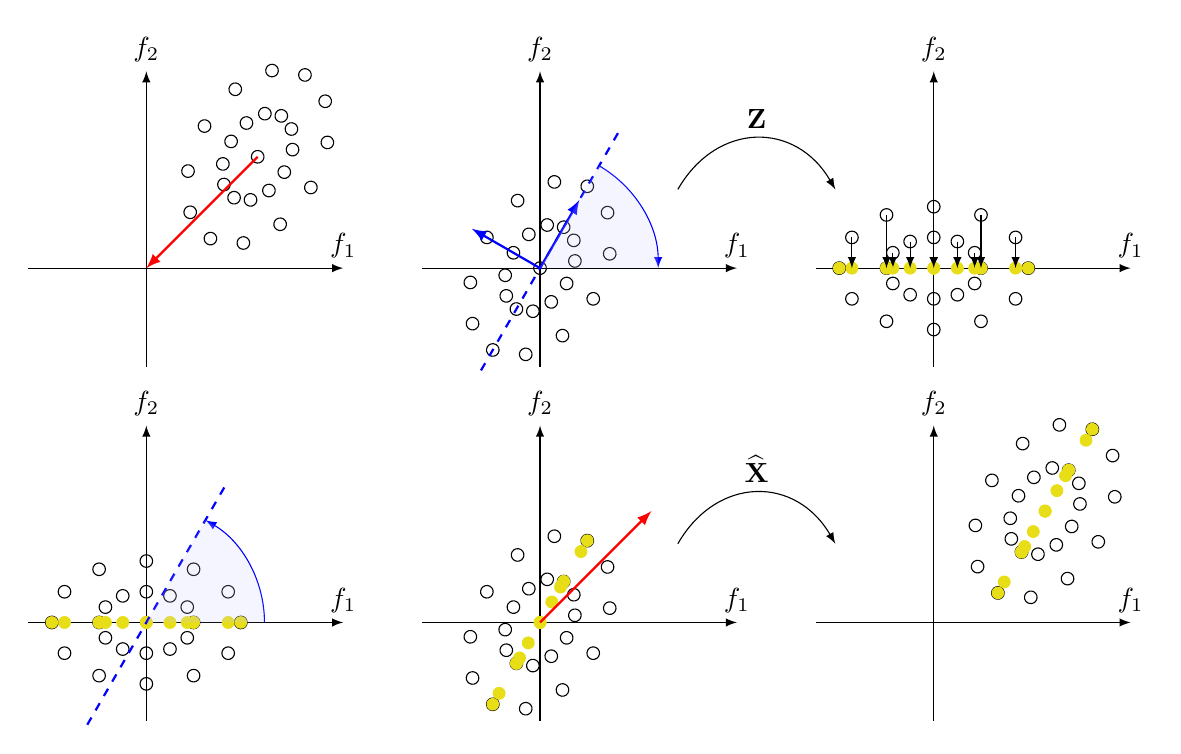
\begin{tikzpicture}[> = latex]

    \def\r{0.08}
    \def\drawAxis{
        \draw [->] (-1.5, 0) -- (2.5, 0) node [above] {$f_1$};
        \draw [->] (0, -1.25) -- (0, 2.5) node [above] {$f_2$};
    }
    \def\drawEllipticalData{
        \draw (0, 0) circle (\r);
        \foreach \mag in {0.6, 1.2}{
            \foreach \ang in {0, 30,..., 330}{
                \draw ({\mag * cos(\ang)}, {0.65 * \mag * sin(\ang)}) circle (\r);
            }
        }
    }
    \def\drawProjections{
        \fill [yellow!90!black] (0, 0) circle (\r);
        \foreach \mag in {0.6, 1.2}{
            \foreach \ang in {0, 30,..., 330}{
                \draw ({\mag * cos(\ang)}, {0.65 * \mag * sin(\ang)}) circle (\r);
                \fill [yellow!90!black] ({\mag * cos(\ang)}, 0) circle (\r);
            }
            \foreach \ang in {30, 60, ..., 150}{
                \draw [->] ({\mag * cos(\ang)}, {0.65 * \mag * sin(\ang)}) -- ({\mag * cos(\ang)}, 0);
            }
        }
    }
    \def\drawProjectionsNoArrows{
        \fill [yellow!90!black] (0, 0) circle (\r);
        \foreach \mag in {0.6, 1.2}{
            \foreach \ang in {0, 30,..., 330}{
                \draw ({\mag * cos(\ang)}, {0.65 * \mag * sin(\ang)}) circle (\r);
                \fill [yellow!90!black] ({\mag * cos(\ang)}, 0) circle (\r);
            }
        }
    }

    % Original data
    \drawAxis
    \begin{scope}[shift={(45:2)}, rotate=60]
        \drawEllipticalData
    \end{scope}
    % Centroid
    \draw [->, thick, red] (45:2) -- (0:0);

    % Zero mean data
    \begin{scope}[shift={(5, 0)}]
        \drawAxis
        \begin{scope}[rotate=60]
            \drawEllipticalData
        \end{scope}
        % Orthonormal eigenvectors
        \draw [dashed, thick, blue] (60:-1.5) -- (60:2); % direction of v1
        \draw [->, thick, blue] (0:0) -- (60:1); % v1
        \draw [->, thick, blue] (0:0) -- (60+90:1); % v2

        % Rotation
        \draw [->, blue] (60:1.5) arc (60:0:1.5);
        \fill [blue!20, opacity=0.2]
            (0:0) -- (60:1.5) arc (60:0:1.5) -- cycle
        ;
    \end{scope}

    \draw [->] 
        (6.75, 1) .. controls ++(60:1) and ++(120:1) .. (8.75, 1) 
        node [midway, above] {$\mathbf{Z}$}
    ;

    % Projections onto biggest eigenvector
    \begin{scope}[shift={(10, 0)}]
        \drawAxis
        % \drawEllipticalData

        % Projections
        \drawProjections
    \end{scope}

    % Reconstructions: rotation
    \begin{scope}[shift={(0, -4.5)}]
        \drawAxis
        % \drawEllipticalData

        % Projections
        \drawProjectionsNoArrows

        % Orthonormal eigenvectors
        \draw [dashed, thick, blue] (60:-1.5) -- (60:2); % direction of v1

        % Rotation
        \draw [<-, blue] (60:1.5) arc (60:0:1.5);
        \fill [blue!20, opacity=0.2]
            (0:0) -- (60:1.5) arc (60:0:1.5) -- cycle
        ;
    \end{scope}

    % Reconstructions: translation
    \begin{scope}[shift={(5, -4.5)}]
        \drawAxis

        \begin{scope}[rotate=60]
            \drawProjectionsNoArrows
        \end{scope}

        \draw [<-, thick, red] (45:2) -- (0:0);
    \end{scope}

    \draw [->] 
        (6.75, 1-4.5) .. controls ++(60:1) and ++(120:1) .. (8.75, 1-4.5) 
        node [midway, above] {$\widehat{\mathbf{X}}$}
    ;

    % Reconstructions: results
    \begin{scope}[shift={(10, -4.5)}]
        \drawAxis

        \begin{scope}[shift={(45:2)}, rotate=60]
            \drawProjectionsNoArrows
        \end{scope}
    \end{scope}
\end{tikzpicture}
\end{figure}

Note that by defining the $n \times d$ matrices 
$\overline{X}_{ij} = \overline{X}_j$ and
$S_{ij} = S_j$,
$\mathbf{Y}$ can be handily given as two pointwise operations,
$\mathbf{Y} = (\mathbf{X}-\overline{\mathbf{X}}) / \mathbf{S}$.

Now, for the dataset in question, the following values were observed%
\footnote{%
    See the \texttt{.csv} files in folder \texttt{results/pca/} inside the code zip.
}:
%
\begin{alignat}{3}
    X_1 &= 2.523,\quad& X_2 &= -2.813,\quad& X_3 &= 0.304 \\
    S_1 &= 1.408,\quad& S_2 &=  5.379,\quad& S_3 &= 9.365
\end{alignat}

Which lead to the following correlation matrix:
%
\begin{equation}
    \mathbf{W} = 
    \begin{bmatrix}
         1.000 & -0.534 & -0.607 \\
        -0.534 &  1.000 &  0.941 \\
        -0.607 &  0.941 &  1.000 
    \end{bmatrix}
\end{equation}

The orthonormal eigenvectors associated with $\mathbf{W}$ and associated eigenvalues are presented below.
%
\begin{alignat}{3}
    \mathbf{v}_1 =&
    \begin{bmatrix}
         0.498 \\
        -0.605 \\
        -0.621
    \end{bmatrix}, \quad
    &
    \mathbf{v}_2 =& 
    \begin{bmatrix}
        -0.863 \\
        -0.416 \\
        -0.287
    \end{bmatrix}, \quad
    &
    \mathbf{v}_3 =& 
    \begin{bmatrix}
        0.085 \\
        -0.678 \\
        0.730
    \end{bmatrix}, \quad
    \\
    \alpha_1 =& 2.406, \quad &
    \alpha_2 =& 0.542, \quad &
    \alpha_3 =& 0.056 
    \\
    &(80.116\ \%) & 
    &(18.034\ \%) & 
    &(1.859\ \%) 
\end{alignat}

The values in parentheses represent the weight of the eigenvector 
in reconstructions of data from PCA, i.e., 
the value of the associated eigenvalue divided by the sum of all eigenvalues.
%
In turn, the 1D, 2D, and 3D reconstructions of $\mathbf{X}$ using the calculated eigenvectors 
are given by the following equations:
%
\begin{align}
    \widehat{\mathbf{X}}_{1D} &= (\mathbf{y}_1\mathbf{v}_1^T) \circ \mathbf{S} + \overline{\mathbf{X}} \\
    \widehat{\mathbf{X}}_{2D} &= \mathbf{X}_{1D} + (\mathbf{y}_2\mathbf{v}_2^T) \circ \mathbf{S} \\
    \widehat{\mathbf{X}}_{3D} &= \mathbf{X}_{2D} + (\mathbf{y}_3\mathbf{v}_3^T) \circ \mathbf{S} 
\end{align}
%
where $\circ$ denotes the Hadamard (i.e., pointwise) product and 
$\widehat{\mathbf{X}}_{3D}$ is exactly equal to the original data.

These results indicate that $\mathbf{v}_1$ is, by far, 
the most representative direction of spread of data,
although $\mathbf{v}_2$ also hold meaningful weight.
Conversely, the smallest vector $\mathbf{v}_3$ contributes very little information
into the reconstructions, and should be safely excluded in PCA.

In light of this brief analysis, it is concluded that an effective PCA will use only 
$\mathbf{v}_1$ and $\mathbf{v}_2$, dropping one dimention from the original dataset.
%
The figure below shows the original data \textit{versus} its reconstructions using 
(i) only $\mathbf{v}_1$;
(ii) both $\mathbf{v}_1$ and $\mathbf{v}_2$.
From inspection, it is safe to say that the 2D reconstruction is quite representative of data,
while the 1D is not.
%
As such, PCA, in particular its bidimensional version, should prove a useful tool for simplifying this dataset.

\begin{figure}[htbp]
    \centering
    \caption{
        Original data (black) versus PCA 1D (blue) and 2D (red) reconstructions.
        Bottom row shows the same view angles as top row but at higher elevation.
    }
    \label{fig:pca-reconstructions}
    % Top row of plots
    \begin{subfigure}[t]{.24\textwidth}
        \centering
        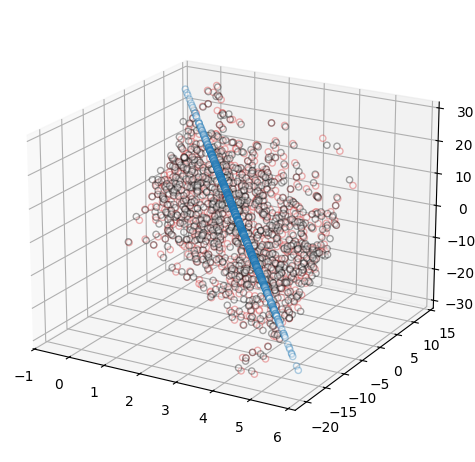
\includegraphics[width=\linewidth]
        {../../python_code/plots/pca/pca_reconstructions_elev20_azim-60.png}
    \end{subfigure}
    \begin{subfigure}[t]{.24\textwidth}
        \centering
        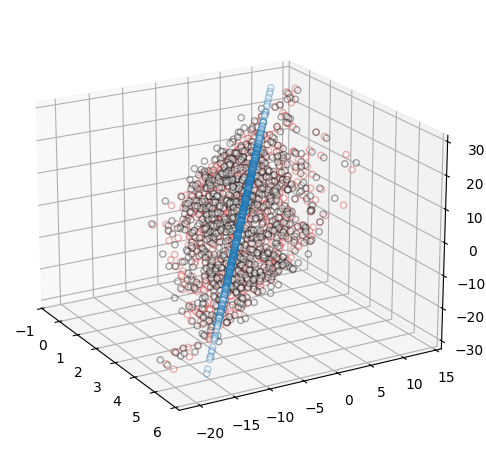
\includegraphics[width=\linewidth]
        {../../python_code/plots/pca/pca_reconstructions_elev20_azim-30.png}
    \end{subfigure}
    \begin{subfigure}[t]{.24\textwidth}
        \centering
        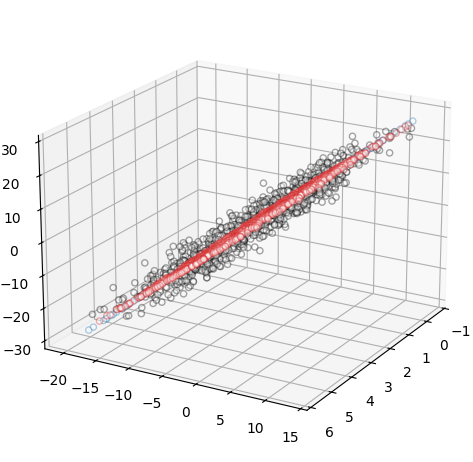
\includegraphics[width=\linewidth]
        {../../python_code/plots/pca/pca_reconstructions_elev20_azim30.png}
    \end{subfigure}
    \begin{subfigure}[t]{.24\textwidth}
        \centering
        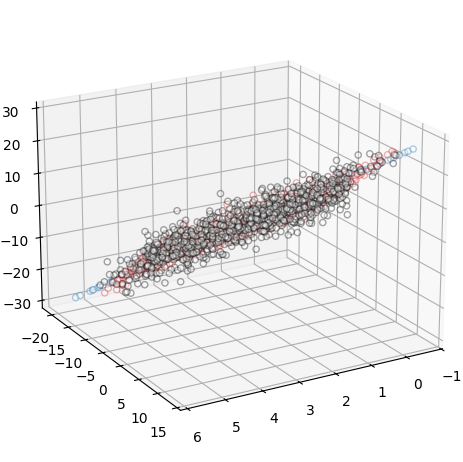
\includegraphics[width=\linewidth]
        {../../python_code/plots/pca/pca_reconstructions_elev20_azim60.png}
    \end{subfigure}
    % Second row of plots
    \begin{subfigure}[t]{.24\textwidth}
        \centering
        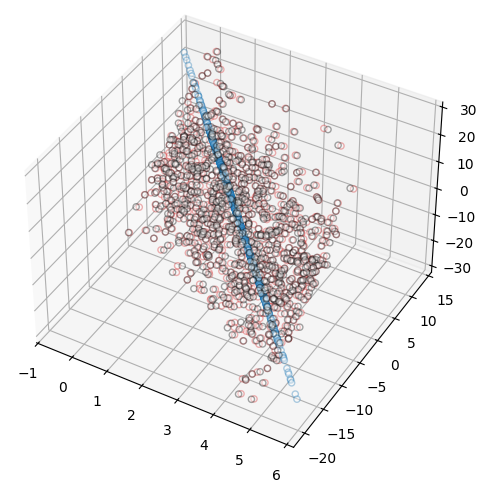
\includegraphics[width=\linewidth]
        {../../python_code/plots/pca/pca_reconstructions_elev40_azim-60.png}
    \end{subfigure}
    \begin{subfigure}[t]{.24\textwidth}
        \centering
        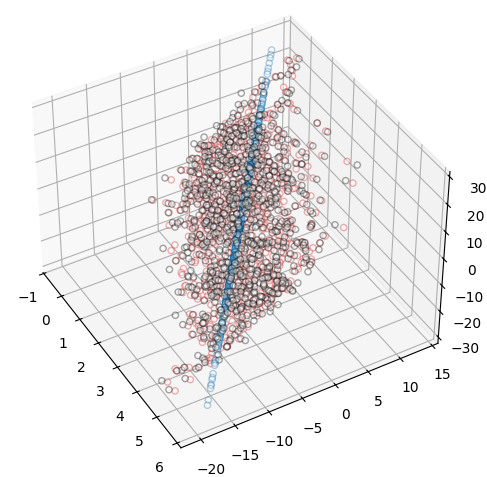
\includegraphics[width=\linewidth]
        {../../python_code/plots/pca/pca_reconstructions_elev40_azim-30.png}
    \end{subfigure}
    \begin{subfigure}[t]{.24\textwidth}
        \centering
        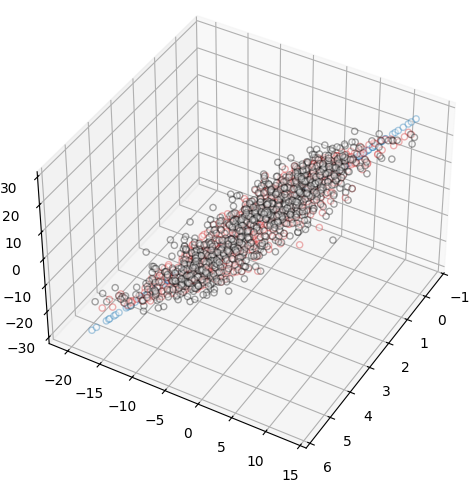
\includegraphics[width=\linewidth]
        {../../python_code/plots/pca/pca_reconstructions_elev40_azim30.png}
    \end{subfigure}
    \begin{subfigure}[t]{.24\textwidth}
        \centering
        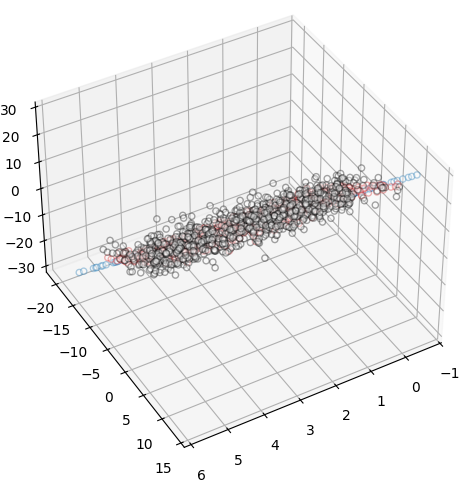
\includegraphics[width=\linewidth]
        {../../python_code/plots/pca/pca_reconstructions_elev40_azim60.png}
    \end{subfigure}
    % Bottom row of plots
    \begin{subfigure}[t]{.24\textwidth}
        \centering
        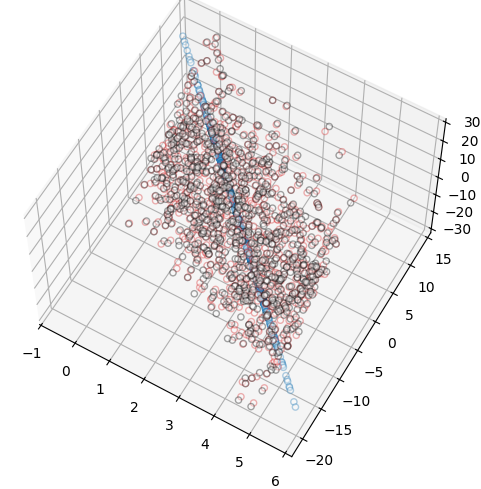
\includegraphics[width=\linewidth]
        {../../python_code/plots/pca/pca_reconstructions_elev60_azim-60.png}
    \end{subfigure}
    \begin{subfigure}[t]{.24\textwidth}
        \centering
        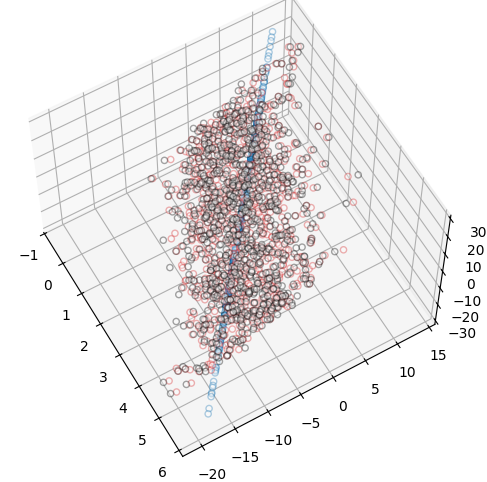
\includegraphics[width=\linewidth]
        {../../python_code/plots/pca/pca_reconstructions_elev60_azim-30.png}
    \end{subfigure}
    \begin{subfigure}[t]{.24\textwidth}
        \centering
        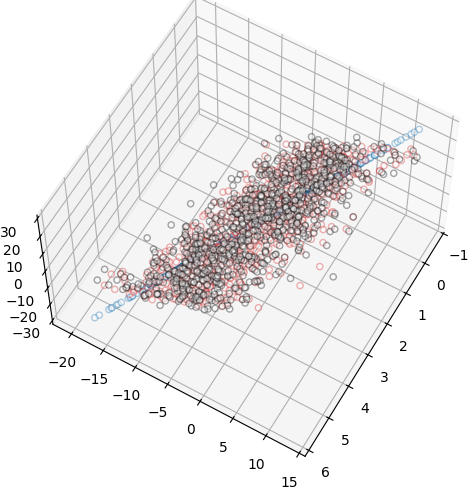
\includegraphics[width=\linewidth]
        {../../python_code/plots/pca/pca_reconstructions_elev60_azim30.png}
    \end{subfigure}
    \begin{subfigure}[t]{.24\textwidth}
        \centering
        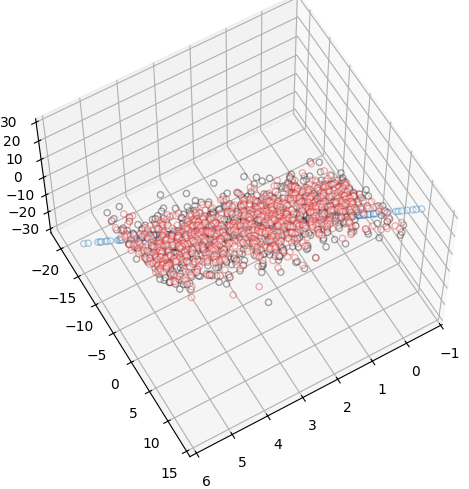
\includegraphics[width=\linewidth]
        {../../python_code/plots/pca/pca_reconstructions_elev60_azim60.png}
    \end{subfigure}
\end{figure}
